\documentclass{sigchi-ext}

\usepackage[T1]{fontenc}
\usepackage{textcomp}
\usepackage[scaled=.92]{helvet} % for proper fonts
\usepackage{graphicx} % for EPS use the graphics package instead
\usepackage{balance}  % for useful for balancing the last columns
\usepackage{booktabs} % for pretty table rules
\usepackage{ccicons}  % for Creative Commons citation icons
\usepackage{ragged2e} % for tighter hyphenation
\usepackage[utf8]{inputenc} 

\def\plaintitle{SIGCHI Extended Abstracts Sample File: Note Initial
  Caps} \def\plainauthor{First Author, Second Author}
\def\emptyauthor{}
\def\plainkeywords{Neurodevelopmental Disorders; children; virtual reality; learning; game; nutrition; autonomy; food pyramid.}
\def\plaingeneralterms{Documentation, Standardization}

\title{GEA - a VR Game for Nutrition Education for Children with Neurodevelopmental Disorders}

\numberofauthors{5}

\author{%
	\vspace{20px}
    \textbf{Federica Blanco}\\
    \textbf{Giulia Pennati}\\
    \textbf{Vito Matarazzo}\\
    \textbf{Nicolò Messina}\\
    \textbf{Franca Garzotto}\\
    %\vspace{70px}
    \affaddr{Department of Electronics, Information and Bioengineerin}\\
    \affaddr{Politecnico di Milano} \\
    \affaddr{20133 Milano, Italy} \\
    $\{$federica.blanco, giulia1.pennati$\}$@mail.polimi.it\\
    $\{$vito.matarazzo, nicolo.messina, franca.garzotto$\}$@polimi.it
    }

\definecolor{linkColor}{RGB}{6,125,233}
\hypersetup{%
  pdftitle={\plaintitle},
%  pdfauthor={\plainauthor},
  pdfauthor={\emptyauthor},
  pdfkeywords={\plainkeywords},
  bookmarksnumbered,
  pdfstartview={FitH},
  colorlinks,
  citecolor=black,
  filecolor=black,
  linkcolor=black,
  urlcolor=linkColor,
  breaklinks=true,
}

% \reversemarginpar%

\begin{document}

%% For the camera ready, use the commands provided by the ACM in the Permission Release Form.
%\CopyrightYear{2007}
%\setcopyright{rightsretained}
%\conferenceinfo{WOODSTOCK}{'97 El Paso, Texas USA}
%\isbn{0-12345-67-8/90/01}
%\doi{http://dx.doi.org/10.1145/2858036.2858119}
%% Then override the default copyright message with the \acmcopyright command.
%\copyrightinfo{\acmcopyright}

\maketitle

\RaggedRight{} 


\begin{abstract}
  	This document describes the design of GEA, a web application for children with Neurodevelopmental Disorders that has been designed in collaboration with a team of therapists and children themselves. GEA wants to teach nutrition education through a virtual reality game focused on recognizing the right food for the right situation and avoiding wastes. It is based on real laboratory activities that children do in a local specialized center. We have reproduced these activities in a smart and comfortable space, in which children can play the three different games proposed. The application allows to choose the level of difficulty, in order to customize the game based on each child’s skills. GEA has also a functionality that replicates the smartphone screen on an external device so that the therapists can see what the child is doing and provide help if there are some difficulties. 
\end{abstract}

\keywords{\plainkeywords}
\section{ACM Classification Keywords}
$\bullet$\textbf{Human-centered computing$\sim$Virtual reality}
$\bullet$\textbf{Social and professional topics$\sim$People with disabilities}
$\bullet$\textit{Social and professional topics$\sim$Children} 
$\bullet$\textit{Applied computing$\sim$Interactive learning environments}



\section{Introduction}
\marginpar{
  \vspace{50pt} 
    \begin{minipage}{0.925\marginparwidth}
  	  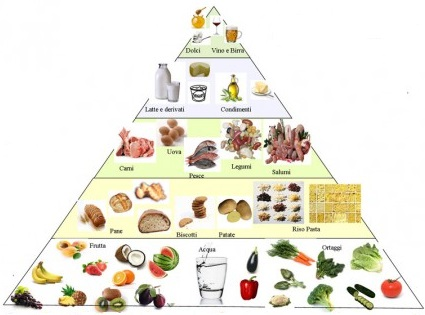
\includegraphics[width=\marginparwidth, height=90px]{figures/piramide.jpg}
  	  \captionof{figure}{The food pyramid, representing the optimal quantity of food to be eaten each day from each of the basic food groups}
      \label{fig:piramide}
      %\vspace{30pt}
      %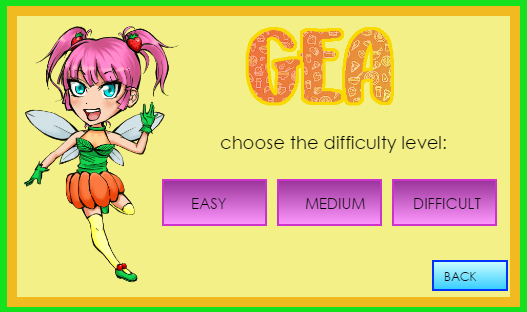
\includegraphics[width=\marginparwidth, height=90px]{figures/Level.png}
  	  %\captionof{figure}{GEA levels of difficulty }
      %\label{fig:levels}
    \end{minipage}}
Neurodevelopmental Disorders (NDD) is an umbrella term for a group of disabilities caused by a dysfunction of a part of the brain or of the nervous system and show their symptoms in the children’s physical and psychological development \cite{rif1}. Examples of this group of disorders are Autism Spectrum Disorder (ASD) Attention Deficit and Hyperactivity Disorder (ADHD) and Down syndrome \cite{rif2}. Children suffering from these syndromes need help in developing cognitive abilities such as attention and language, social skills such as the ability to relate to others and personal and domestic autonomies.
\\
\medskip
Virtual Reality (VR) is nowadays easy to access because it requires the use of a smartphone, owned by the majority of the population, and a VR headset available at low cost; moreover, this technology has been much improved, so that the problems of past generation devices, such as weight and motion sickness \cite{rif6}, have been greatly reduced. The are many studies that applied VR in educational and rehabilitation contexts, comparing this technological approach with the traditional methods and highlighting potential benefits \cite{rif3} \cite{rif4} \cite{rif5}. The interest in VR is therefore increased also in the field of NDD \cite{rif7} \cite{rif8}.
\\
\medskip
Our project falls in this area, since it aims to help children with NDD, through the use of the VR technology, in developing their autonomy and knowledge in the field of nutrition, of great importance nowadays as demonstrated during the recent Expo held in Milan \cite{rif9}.
Thanks to the developed games, children can train their memory by remembering the different levels of the food pyramid (Figure \ref{fig:piramide}), they can learn to distinguish healthy foods from the so-called "junk foods" and can understand how to associate a meal of the day with a dish and vice versa.

    
\section{Approach}
Our application is named GEA (Gioco Educazione Alimentare, Italian words for “Food Education Game”) and has been co-designed with NDD specialists from a local therapeutic center called \emph{Fraternità e Amicizia}. They asked us to transform the food laboratory they propose to children once a week with the presence of a specialist in an interactive digital game. In this laboratory,they perform activities such as creating a billboard with the food pyramid and pasting dishes images or cutting out unhealthy foods from a supermarket flyer. \\
\medskip
The creation of a learning game in VR may bring many benefits: children are usually attracted by new technologies such as VR, and the use of wearable headsets helps maintain attention and concentration since it removes the distractions of the external world. Moreover, VR devices are easy to use, as they require little knowledge of the technology behind them, and they allow to reproduce the real environment of the therapy, facilitating the familiarization with the game.\\ 
\medskip
Among the various types of VR viewers available today, we decided to use Google Cardboard, the cheapest solution on the market, since the game is meant to be integrated in existing therapeutic programs and widely adopted. This viewer is composed of two biconvex lenses mounted on a plastic or cardboard structure available in different colors and shapes. The smartphone set inside this structure displays the visual contents, splitting them into two near-identical bi-dimensional images, and the interaction is achieved through gaze focus. The user can navigate in the virtual world by rotating his/her head, which will consequently rotate the virtual scene projected in the display.\\
\medskip
The effectiveness of learning by playing also lies in the ability to personalize the game based on the abilities of the individual user: for this reason, three different levels of difficulty have been inserted, among which the therapist can decide according to the specific patient’s needs and capabilities. We have also decided to divide GEA into three different activities, as the specialists pointed out the fact that each user has more difficulties in learning one concept than another; therefore, the therapists can decide which activity to propose to their patient in each session.



\section{GEA: Requirements}
\marginpar{
  \vspace{-30pt} 
    \begin{minipage}{0.925\marginparwidth}
  	  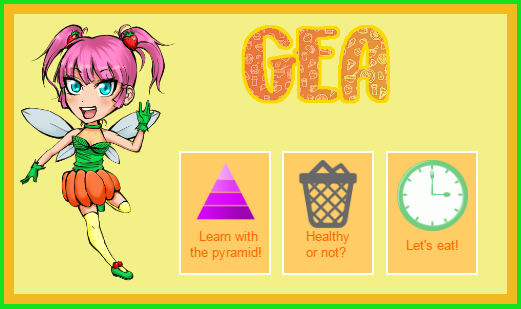
\includegraphics[width=\marginparwidth, height=90px]{figures/Game.png}
  	  \captionof{figure}{GEA home page}
      \label{fig:home page}
      \vspace{30pt}
      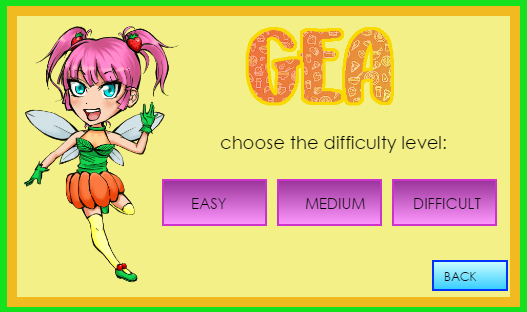
\includegraphics[width=\marginparwidth, height=90px]{figures/Level.png}
  	  \captionof{figure}{GEA levels of difficulty }
      \label{fig:levels}
    \end{minipage}}
The requirements for GEA were collected through meetings with psychologists and experts in the field of NDD. We also took part to some of the food laboratory activities organized in the therapeutic center collaborating with us. We observed how the activities are performed and we discussed with the patients (children and young adults) and the therapists of the center about the idea of realizing a VR game with the same contents and goal. Moreover, we asked them questions about what they like of the food laboratory, what are the difficulties they usually encounter, what is the patients’ relationship with technology and what they would expect from a VR game. After these meetings, we extracted the following requirements for the application to be realized:
\begin{enumerate}
\item \textit{Requirement 1: Customization}\\
      The therapist must be able to set a level of difficulty in the game based on the child’s skills so as to adapt the game to his/her level of knowledge and then gradually increase the difficulty.
\item \textit{Requirement 2: Inherent contents}\\
	  The contents of the game must be inherent and reflect those used during the food laboratory workshops. For this reason, the developed games should be based on the food pyramid, on the recognition of healthy foods and on the ability to associate dishes and meals.
	  \medskip
\item \textit{Requirement 3: Simple virtual environment}\\
	  Because of the various disabilities possessed by users, particular attention to the visualized graphics should be kept: the environment should contain only elements essential for the specific task and cold colors should be avoided, as well as unexpected or flashing animations, as they could trigger negative reactions in the users.
\item \textit{Requirement 4: Visual explanations}\\
	  The possible users of the game differ in age and severity of disability, so there is the possibility that not everyone can read. For this reason, each task must include visual explanations about the goal of the game and how to complete it.
\item \textit{Requirement 5: Importance of Feedback}\\
	  Every user’s action during the game must receive the right feedback. Giving a positive feedback when the right action is accomplished and a negative one when a mistake is made helps maintain the children attention span and their engagement in the game.
\item \textit{Requirement 6: Session monitoring}\\
		The therapist must always keep under control what the child is doing during the game experience, in order to follow his/her improvements and difficulties and to be able to provide the necessary explanations. 	  
\end{enumerate}

\section{GEA: Design}
Starting from the above requirements, we designed GEA as an easy-to-use smartphone application including an initial menu,
\begin{figure*}
 \begin{minipage}[c]{\columnwidth}
   \centering
   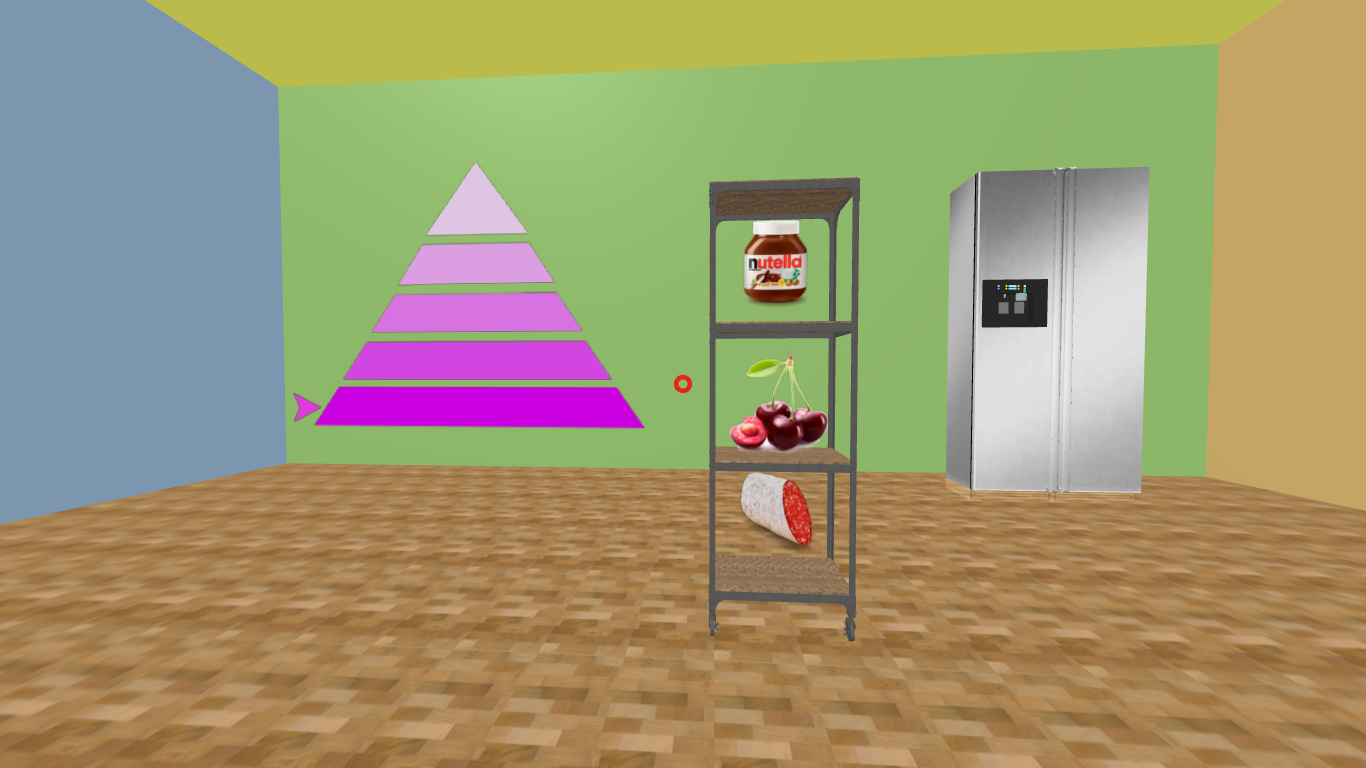
\includegraphics[width=8cm]{figures/Pyramid1.png}
   \caption{"Learn with the pyramid"}
   \label{fig:Pyramid}
 \end{minipage}
 \ \hspace{2mm} \hspace{3mm} \
 \begin{minipage}[c]{\columnwidth}
  \centering
   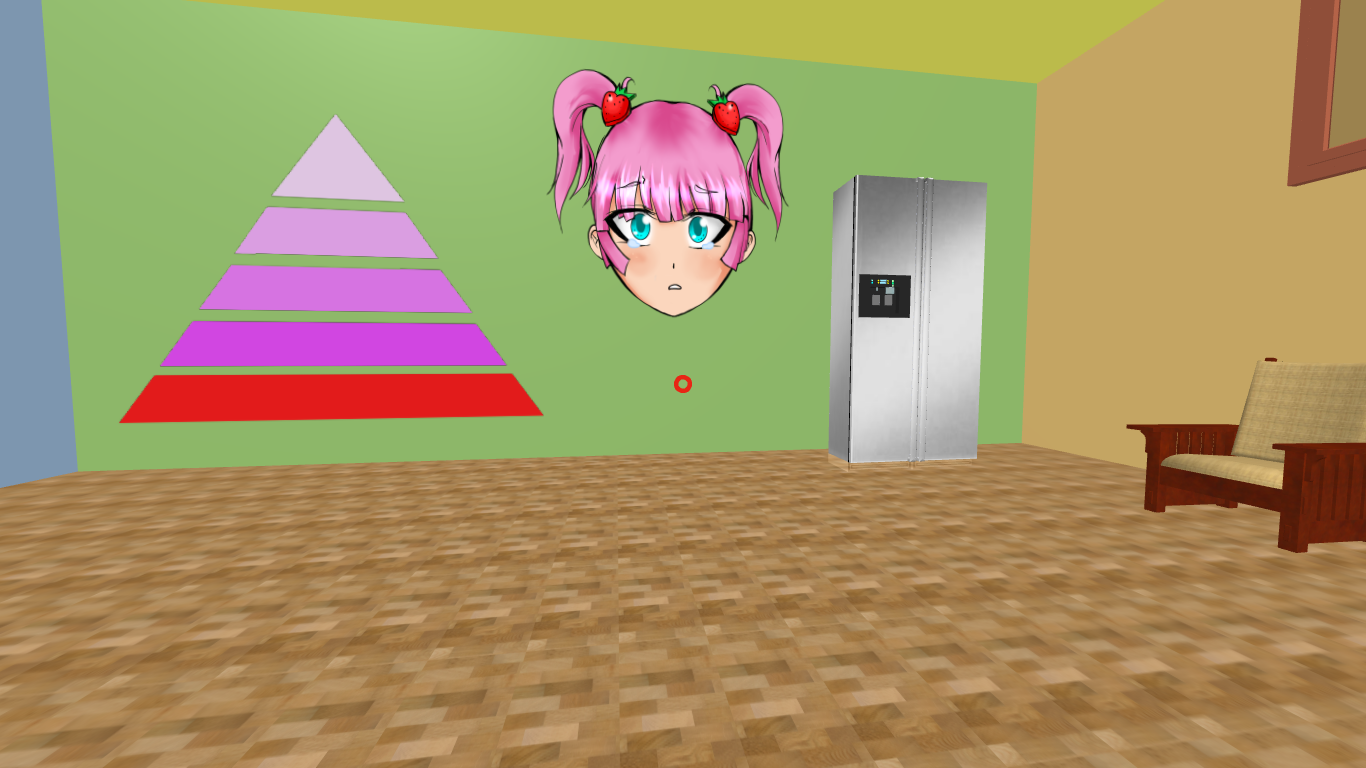
\includegraphics[width=8cm]{figures/Wrong.png}
   \caption{Wrong answer}
   \label{fig:wrong}
 \end{minipage}
\end{figure*}
 from which the therapist can select which game to launch and its level of difficulty, and three VR games, based on the real activities of the previously cited food laboratory. When the application starts, the home page is shown, with the three available games, as shown in Figure \ref{fig:home page}, "Learn with the pyramid!", "Healthy or not?" and "Let’s eat!”. After that, the therapist chooses the level of difficulty of the selected game (Figure \ref{fig:levels}). The difficulty does not lie in the way the game is played or in its objective but in the type of food shown, for example in the easy level you will find common foods such as pasta, pizza or cake while in the difficult level there will be foods such as barley, chickpeas and papaya that are less known by children. The choice of the game and the difficulty is made via touchscreen on the smartphone, before inserting it in the VR viewer: in this way, the therapist can easily setup the experience before putting the patient in the virtual environment.
 \marginpar{
  \vspace{-190pt} 
    \begin{minipage}{0.925\marginparwidth}
  	  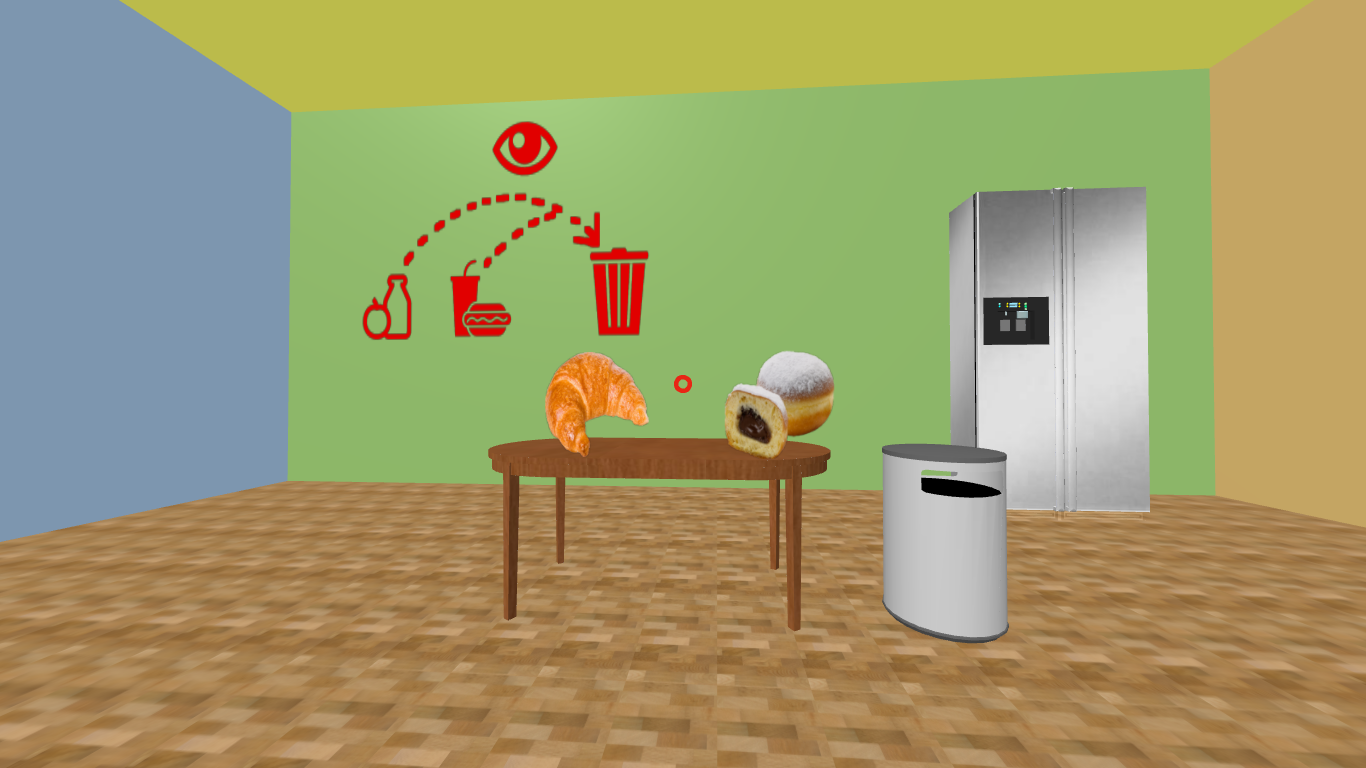
\includegraphics[width=\marginparwidth, height=90px]{figures/Healthy.png}
  	  \captionof{figure}{"Healthy or not?"}
      \label{fig:healthy}
      \vspace{30pt}
      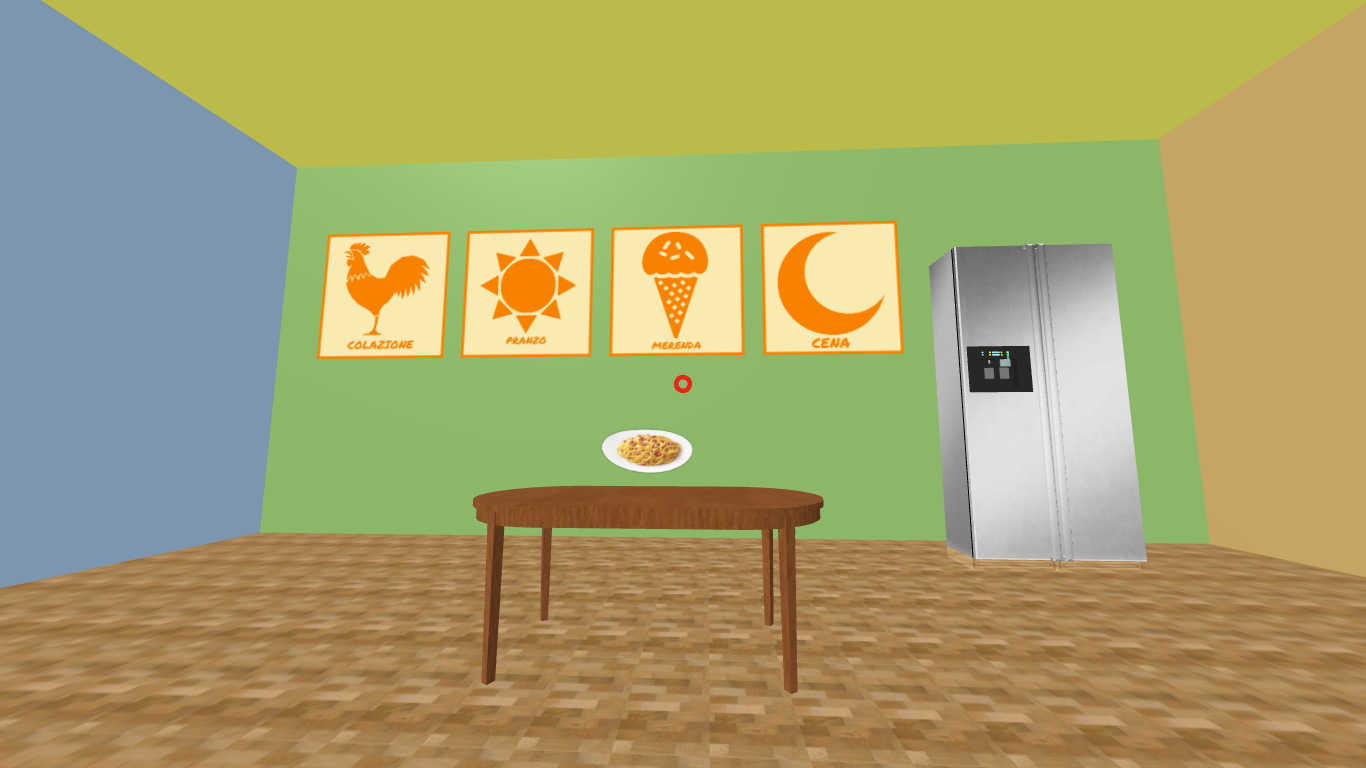
\includegraphics[width=\marginparwidth, height=90px]{figures/Eat.png}
  	  \captionof{figure}{"Let's eat!"}
      \label{fig:eat}
    \end{minipage}}
When the game starts, the patient is immersed in the virtual space, which is the same for all the games and reproduces the real setting of the therapy: there is a room with a table, a fridge, a window, a door, a sofa and a kitchen, in order to keep the space as simple as possible but also inherent with nutrition. In front of the user, a short explanation for each game and a play button appear. The explanation is represented by graphical clues, to be understandable also by users who cannot read.
Moreover, a fantasy character serving as mascot of the game (shown in Figure \ref{fig:home page}) was created, with the goal of making the application more fun and serving as visual feedback after each user’s action.\\ 
\medskip
\textit{\textbf{"Lear with the pyramid!"}}: this game aims to teach how to complete the food pyramid, by selecting which food goes in each level. In the virtual environment the table is substituted by a pyramid divided into five levels, with a pointer indicating which level the user is currently completing and a shelf with three options (Figure \ref{fig:Pyramid}). The red circle in the image is the pointer representing the current user’s focus point. The user has to focus on the correct choice for a certain time interval to give the answer, avoiding possible unwanted answers while the user is looking around in the environment. After an answer is given a feedback appears (Figure \ref{fig:wrong}): the game mascot appears with a sad expression if the answer is wrong and the active level of the pyramid becomes red, if the answer is correct a happy mascot is shown and the level becomes green.\\
\medskip

\textit{\textbf{"Healthy or not?"}}: this game is proposed to train patients in recognizing if a dish is healthy or not. When the game starts, two dishes appear on the table of the virtual room, with a bin and the visual explanation of how the game works (Figure \ref{fig:healthy}): the user must select the “junk food” with the eyes and move it, by keeping the gaze focused on it, until it is thrown in the bin. There are three repetitions of this game, with different choices, and after each answer a feedback is shown, like the one described before.\\
\medskip
\textit{\textbf{"Let's eat!"}}: this game aims to teach how to associate meals of the day to specific dishes. It was created in particular for those patients who have difficulties in understanding when they can eat something or they cannot. In this case, the virtual environment presents four images representing the four main meals (breakfast, lunch, afternoon snack and dinner) and a dish (Figure \ref{fig:eat}): the goal is to select the correct meal/s in which the dish can be eaten. The choice can be also the opposite (selecting which dish corresponds to a certain meal). Like in the second game, there are three repetitions and after each answer a feedback is given.\\
\medskip
At the end of each session with each game the number of correct and wrong answers is shown to the user, with the total scored points.\\
\medskip
The therapist can see what the child is doing in the virtual environment by using a screen casting method, such as Google Chromecast \footnote{https://chromecast.com} , which allows the replication of the smartphone’s screen on an external monitor.


\section{GEA: Implementation}
GEA has been developed as web applications, which ensures a high degree of portability on any platform. We used standard web languages: HTML, JavaScript (for the client side) and PHP (for the server side), with the addition of A-Frame \footnote{https://aframe.io/} , an open-source web framework for creating 3D and virtual reality applications for the web.

\section{Conclusions and future work}
Transforming traditional learning and therapeutic activities for children with NDD into interactive virtual experiences may bring new benefits in this field. VR provides a safe and controllable environment, in which children can train their cognitive and memory skills without possible distractions and with the supervision of a therapist. The increasingly low-cost of VR viewers facilitates a large-scale adoption of this type of applications, while the portability and ease of use of VR technology allows children to perform the same learning activities offered by specialized centers at any time. Using GEA, they can continue their food education with their parents at home, without having to wait for the dedicated laboratory at the therapeutic center.\\
Moreover, the availability on the Internet allows the application to rely upon a large database of game contents, which can be extended at any time by the therapists, making the game activities virtually infinite. Finally, the presence of simple and colorful graphics makes the game more fun, motivating children in learning by playing.\\
\medskip
Our future work in the short term includes the execution of an empirical study at the therapeutic center collaborating with us. The goal of this study is to verify the learning benefits of the developed VR games, comparing the results with the traditional laboratory activity. Additionally, the application will be improved with new functionalities, suggested by the therapists collaborating with us. For example, the possibility for the therapist to interact during the activity, by pausing the game at any time to give children explanations and suggestions if needed. A further development can be to add new themes for the application games, such as a game about allergies, teaching children how to identify what they can eat and what they cannot.

%\section{References Format}
\renewcommand\refname{ciao}
\begin{thebibliography}{100}
\bibitem{rif1} EPA, "United States Environmental Protection Agency". America’s Children and the Environment | Third Edition, Updated October 2015. 
\url{https://www.epa.gov/sites/production/files/2015-10/documents/ace3_neurodevelopmental.pdf}
\bibitem{rif2} American Psychiatric Association, 2013. Diagnostic and statistical manual of mental disorders (DSM-5®). American Psychiatric Pub. 
\bibitem{rif3} Trevor Hall, Lin Lin, Fabrizia Mantovani, Nigel Newbutt, Thomas D. Parsons, Sarah Parsons, Giuseppe Riva, Eva Venturini, . "Virtual Reality in Pediatric Psychology" 
\url{http://pediatrics.aappublications.org/content/ pediatrics/140/Supplement_2/S86.full.pdf}
\bibitem{rif4} Denise Reid, Michelle Wang. "Virtual Reality in Pediatric Neurorehabilitation:Attention Deficit Hyperactivity Disorder, Autism and Cerebral Palsy" 
\url{https://www.karger.com/Article/Pdf/320847} 
\bibitem{rif5} "Effectiveness of virtual reality using Wii gaming technology in children with Down syndrome", Research in Developmental Disabilities Volume 32, Issue 1, January–February 2011, Pages 312-321
\bibitem{rif6} Strickland, D. C., Marcus, L. M., Mesibov, G. B., Hogan, K. 1996. Brief report: Two case studies using virtual reality as a learning tool for autistic children.Journal of Autism and Developmental Disorders, 26(6), 651–659  
\bibitem{rif7} Franca Garzotto, Mirko Gelsomini, and Daniele Occhiuto. 2016 (Conference Paper). Wildcard: A Wearable Virtual Reality Storytelling Tool for Children with Intellectual Developmental Disability Annual International Conference of the IEEE Engineering in Medicine and Biology Society (EMBC’16)
\bibitem{rif8} Yufang Cheng, PhD, Cheng-Li Huang, MA, Chung-Sung Yang, PhD. 2015. Using a 3D Immersive Virtual Environment System to Enhance Social Understanding and Social Skills for Children With Autism Spectrum Disorders. Focus on Autism and Other Developmental Disabilities, 30(4), 222–236. DOI:  \url{https://doi.org/10.1177/1088357615583473 }
\bibitem{rif9} EXPO 2015, Milan. \url{www.expo2015.org/}
\end{thebibliography}

\balance{} 
\bibliographystyle{SIGCHI-Reference-Format}
%\bibliography{sample}
\end{document}

%%% Local Variables:
%%% mode: latex
%%% TeX-master: t
%%% End:
